\documentclass[addpoints]{exam}

\usepackage[top=2cm, bottom=2cm, left=2cm, right=2cm]{geometry}
\usepackage[utf8]{inputenc}
\usepackage[icelandic]{babel}
\usepackage[T1]{fontenc}
\usepackage[sc]{mathpazo}

\makeatletter % Fix due to (recent versions of?) minted containing their own framed definition
\expandafter\providecommand\expandafter*\csname ver@framed.sty\endcsname
{2003/07/21 v0.8a Simulated by exam}
\makeatother

\usepackage[parfill]{parskip}
\usepackage{booktabs,tabularx}
\usepackage{multirow}
\usepackage{multicol}
\usepackage{graphicx}
\usepackage{enumerate}
\usepackage{amsmath, amsfonts, amssymb, amsthm}
\usepackage{minted} %Minted and configuration
\usepackage{afterpage}
\usepackage{scrextend}

\usepackage[pdftex,bookmarks=true,colorlinks=true,pdfauthor={Eirikur Ernir Thorsteinsson},linkcolor=blue,urlcolor=blue]{hyperref}

\setcounter{secnumdepth}{-1} 
\hyphenpenalty=5000

\newcommand\blankpage{%
    \null
    \thispagestyle{empty}%
    \addtocounter{page}{-1}%
    }

\usemintedstyle{default}
\renewcommand{\theFancyVerbLine}{\sffamily \arabic{FancyVerbLine}}
\author{}
\date{}

\footer{}{}{}

\setcounter{secnumdepth}{-1} 

\qformat{\large \textbf Spurning \thequestion \phantom{M}(\totalpoints \phantom{l}stig) \hfill}
\renewcommand{\solutiontitle}{\noindent\textbf{Svar:}\par\noindent}
\renewcommand{\points}{stig}
\renewcommand{\questionshook}{\setlength{\itemsep}{0.5cm}}
\hqword{Spurning:}
\hpword{Stig í boði:}
\hsword{Stig:}
\htword{Samtals}

\newmintedfile[cppfile]{cpp}{frame=lines, linenos=false}
\newmintedfile[javafile]{java}{frame=lines, linenos=false}
\newcommand{\eng}[1]{(e.\ \emph{#1})}

\title{TÖL203G Tölvunarfræði 2 - lokapróf}
\author{}
\date{28. apríl 2017}

\pagestyle{headandfoot}
\firstpageheader{TÖL203G \\ Tölvunarfræði 2}{Lokapróf}{28. apríl 2017}
\firstpagefooter{}{Bls. \thepage\ af \numpages}{}
\runningfooter{}{Bls. \thepage\ af \numpages}{}
\setlength{\columnsep}{0.5cm}

% \printanswers
\begin{document}

% \thispagestyle{empty}
Fullt nafn: \vspace*{1mm} \hrule

\begin{center}
	\begin{minipage}{.8\textwidth}

		\vspace{5cm}

		\textbf{Leiðbeiningar:} Á þessu prófi eru \numquestions\ spurningar sem samtals gefa \numpoints\ stig. Skrifið svör beint á þessar síður. Ef meira pláss vantar, skrifið á bakhlið viðkomandi síðu. Leyfileg hjálpargögn eru reiknivél og ein A4 blaðsíða af glósum. Dæmi prófsins eru misþung og eru ekki sett fram í erfiðleikaröð.

		\vspace{0.5cm}

		\textbf{Instructions:} This exam has \numquestions\ questions worth a total number of \numpoints\ points. Write your answers on the exam sheets. If you run out of space, write on the overleaf. You may bring a calculator and one A4 sheet of notes to the exam. Some questions are less difficult than others, they are not ordered by difficulty.
	\end{minipage}
\end{center}

\vfill
\begin{center}
	\cellwidth{1.5em}
	\gradetable[h][questions]
\end{center}

\newpage

\begin{questions}

	\section{Efnisspurningar}

	\question[4] Spurningar um grunnatriði C++. Merkið við einn réttan möguleika eða gefið stutt svör. \eng{Questions about C++ fundamentals. Select one choice or give short answers.}

	\begin{parts}
		% \part Gefið er C++ forrit. Hvað skrifar það út? \eng{A C++ program is given. What is its output?}
		% 
		% \begin{minted}[frame=lines]{cpp}
		% #include <iostream>
		% int main() {
		%     int v[] = {3, 2, 1};
		%     int i = 3;
		%     while (v[i] == 0) {
		%         i++;
		%     }
		%     std::cout << v[i] << std::endl;
		%     return 0;
		% }
		% 
		% \end{minted}
		% 
		% \begin{checkboxes}
		%  \choice 0
		%  \choice 1
		%  \choice Forritið fer í endalausa lykkju \eng{The program enters an infinite loop}
		%  \choice Forritið þýðist ekki \eng{The program does not compile}
		%  \choice Virkni forritsins er óskilgreind \eng{The program's behaviour is undefined}
		% \end{checkboxes}

		\part Gefinn er C++ forritsbútur. Hvert er gildi breytunnar \texttt{x} eftir að hann hefur verið keyrður?

		\eng{A C++ program snippet is given. What is the value of the variable \texttt{x} after its execution?}
		\begin{minted}[frame=lines]{cpp}
int v[] = {1, 2, 4};
int x = v[3];
\end{minted}

		\begin{checkboxes}
			\choice 0
			\choice 4
			\choice Forritið hrynur við keyrslu \eng{The program crashes at runtime}
			\choice Forritið getur ekki þýðst \eng{The program cannot compile}
			\choice Ómögulegt að segja \eng{It is impossible to tell}
		\end{checkboxes}

		\part Hver eftirfarandi C++ skipana gerir \texttt{b} að bendi á minnissvæði heiltölubreytunnar \texttt{i}?

		\eng{Which of the following C++ statements defines \texttt{b} as a pointer to the memory address of the integer variable \texttt{i}?}

		% \begin{oneparcheckboxes}
		\begin{checkboxes}
			\choice \texttt{\$int b = \&i;}
			\choice \texttt{int* b = \&i;}
			\choice \texttt{int\& b = *i;}
			\choice \texttt{int* b = *i;}
			\choice \texttt{int\& b = \&i;}
		\end{checkboxes}
		% \end{oneparcheckboxes}

		\part Þegar \texttt{new} er notað við skilgreiningu á C++ breytu, í hvaða minnissvæði er breytan geymd? Gerum ráð fyrir kunnuglegum C++ útfærslum.

		\eng{When \texttt{new} is used when defining a variable in C++, where will the variable be stored? Assume a familiar C++ implementation.}

		\begin{checkboxes}
			\choice Í þulu \eng{in the code segment}
			\choice í gagnasvæði \eng{in the data segment}
			\choice Á hlaða \eng{on the stack}
			\choice Í kös \eng{on the heap}
			\choice Á segulbandi \eng{on a tape}
		\end{checkboxes}

		\part Nefndu mögulega ástæðu sem C++ forritari gæti haft til að láta fall taka inn bendi á breytu frekar en breytuna sjálfa.

		\eng{Name a reason why a C++ programmer might write a function that accepts a pointer to a variable rather than the variable itself?}

		\vspace*{1cm} \hrule \vspace*{1cm} \hrule \vspace*{1cm} \hrule

	\end{parts}

	\newpage

	\question[4] Spurningar um keyrslutíma. Merkið við einn réttan möguleika eða gefið stutt svör. \eng{Questions about running time. Select one choice or give short answers.}
	\begin{parts}

		\part Eintengdur listi er notaður á skynsaman hátt til að útfæra hlaða. Hver er keyrslutími innsetningar (\texttt{push}) og eyðingar (\texttt{pop}), m.t.t. fjölda staka á hlaðanum?
		\eng{A singly-linked list is used in a sensible way to implement a stack. What is the running time of insertion (\texttt{push}) and deletion (\texttt{pop}), relative to the number of items on the stack}
		\begin{checkboxes}
			\choice Innsetning og eyðing á föstum tíma \eng{Insertion and deletion in constant time}
			\choice Innsetning og eyðing á logratíma \eng{Insertion and deletion in logarithmic time}
			\choice Innsetning á föstum tíma, eyðing á línulegum tíma \eng{Insertion in constant time, deletion in linear time}
			\choice Innsetning á línulegum tíma, eyðing á föstum tíma \eng{Insertion in linear time, deletion in constant time}
			\choice Annaðhvort innsetning eða eyðing á föstum tíma, hin aðgerðin á logratíma \eng{Either insertion or deletion in constant time, the other operation in linear time}
		\end{checkboxes}

		\part Af hvaða stærðargráðu er lágmarksfjöldi aðgerða sem (hefðbundið) quicksort þarf til að raða $N$ staka safni?

		\eng{Of what order is the best-case number of operations used by the (traditional) quicksort algorithm to sort a collection of $N$ items?}

		\begin{checkboxes}
			\choice 1
			\choice $\log N$
			\choice $N$
			\choice $N \log N$
			\choice $N^2$
		\end{checkboxes}

		\part Af hvaða stærðargráðu er hámarksfjöldi aðgerða sem þarf til uppflettingar í nafnatöflu sem útfærð er með rauðsvörtu tré?

		\eng{Of what order is the worst-case number of operations required for lookup in a symbol table implemented using a red-black tree?}

		\begin{checkboxes}
			\choice 1
			\choice $\log N$
			\choice $N$
			\choice $N \log N$
			\choice $N^2$
		\end{checkboxes}

		\part Nefnið eitt dæmi um sérstakar aðstæður þar sem innsetningarröðun er skilvirkari en sameiningarröðun.

		\eng{Specify a situation where insertion sort is more efficient than merge sort.}

		\vspace*{1cm} \hrule \vspace*{1cm} \hrule \vspace*{1cm} \hrule \vspace*{1cm} \hrule

	\end{parts}

	\newpage

	\question[4] Spurningar um net. Merkið við einn réttan möguleika eða gefið stutt svör.
	\eng{Questions about graphs. Select one choice or give short answers.}

	\begin{parts}

		\part Hver er lágmarksfjöldi leggja sem þarf til að tengja saman net með $N$ hnútum svo úr verði net með einum samhengisþætti?

		\eng{What is the minimum number of edges required to connect a graph with $N$ vertices, forming a single connected component?}

		\begin{checkboxes}
			\choice $\log N$
			\choice $N-1$
			\choice $N$
			\choice $N^2$
			\choice $2^N$
		\end{checkboxes}

		\part Hvert eftirfarandi reiknirit má nota til að finna léttasta spanntré nets?

		\eng{Which of the following algorithms can be used to find a minimum spanning tree?}

		\begin{checkboxes}
			\choice Reiknirit Dijkstra \eng{Dijkstra's algorithm}
			\choice Bellman-Ford reikniritið \eng{The Bellman-Ford algorithm}
			\choice Breiddarleit \eng{Breadth-first search}
			\choice Dýptarleit \eng{Depth-first search}
			\choice Reiknirit Prim's \eng{Prim's Algorithm}
		\end{checkboxes}

		\part Útskýrðu með eigin orðum muninn á dýptarleit og breiddarleit.

		\eng{Using your own words, explain the difference between depth-first search and breadth-first search.}

		\vspace*{1cm} \hrule \vspace*{1cm} \hrule \vspace*{1cm} \hrule \vspace*{1cm} \hrule \vspace*{1cm} \hrule

		\part Nefndu ókosti við nota grennslafylki til að að útfæra klasa sem táknar net.

		\eng{Name a drawback of using an adjacency matrix to implement a class representing a graph.}

		\vspace*{1cm} \hrule \vspace*{1cm} \hrule \vspace*{1cm} \hrule \vspace*{1cm} \hrule \vspace*{1cm} \hrule

	\end{parts}

	\newpage

	\section{Forritunarspurningar}

	Í Java forritum má gera ráð fyrir að allir klasar skilgreindir í \texttt{algs4} safni bókarinnar séu aðgengilegir, ekki þarf að skrifa \texttt{import} skipanir. Valin skil eru gefin í viðauka. Í C++ forritum má gera ráð fyrir að \texttt{std} nafnarýmið sé virkt og þekktir hausar (t.d. \texttt{iostream} og \texttt{vector}) séu aðgengilegir, ekki þarf að skrifa \texttt{include} skipanir.

	\eng{When writing Java programs access to all classes in \texttt{algs4.jar} may be assumed, \texttt{import} statements are not required. Selected APIs are given in the appendix. When writing C++ programs the \texttt{std} namespace may be assumed to be active, and common headers (e.g. \texttt{iostream} and \texttt{vector}) can be considered included.}

	\question[4] Skrifið Java-aðferðina \texttt{reverseStack} sem tekur inn hlaða og snýr við röð stakanna sem í honum eru.

	\eng{Write the Java method \texttt{reverseStack} which accepts a stack as its input parameter and reverses its order of items.}

	\begin{minted}[frame=lines]{java}
void reverseStack(Stack<Item> stack) {





































}
\end{minted}


	\question[4] Gefinn er hluti af útfærslu á eintengdum lista tákna í C++ á næstu síðu. Klárið innsetningaraðferð klasans, sem vinnur samkvæmt kóðalýsingunni.

	\eng{A partial singly linked list implementation in C++ is given on the following page. Finish the insertion method according to the code description.}
	\begin{minted}[frame=lines]{cpp}
void insert(int index, char data) {
	/*  index: an integer in the range [0:n]
	 *  data: a single character
	 *  Creates a new Node containing the data at position index in the list.
	 */
	 
	 
	 
	 
	 
	 
	 
	 
	 
	 
	 
	 
	 
	 
	 
	 
	 
	 
	 
	 
	 
	 
	 
	 
	 
	 
	 
	 
	 
	 
	 
	 
	 
	 
	 
	 
	 
	 
	 
	 
	 
	 
	 
}
\end{minted}
	\newpage
	\begin{minted}[frame=lines]{cpp}
class Node {
    /*
     * Represents a node for use in a singly linked list
     */
public:
    char data;
    Node *next;

    Node(char data, Node *next) {
        this->data = data;
        this->next = next;
    }
};


class LinkedList {
    /*
     * Represents a Singly Linked List
     */
private:
    Node *head = nullptr;
    int n = 0;

public:

    void insert(int index, char data) {
        // See previous page
    }

    int size() {
        return this->n;
    }

    bool isEmpty() {
        return this->head == nullptr;
    }
};
\end{minted}


	\newpage

	% \question[4] Gefinn er hluti af útfærslu á hlaða í C++. Klárið að útfæra \texttt{pop()} aðferðina í samræmi við lýsingu í kóðanum.
	% \cppfile{Code/w13/Node.cpp}
	% \cppfile{Code/w13/Stack.cpp}

	%\question[4] Gefinn er hluti af útfærslu á biðröð í C++. Útfærið þær aðferðir sem vantar.

	% \question[4] Skrifið Java-aðferðina \texttt{mergeBags} sem tekur inn tvær skjóður og skilar nýrri skjóðu sem inniheldur gögn inntaksskjóðanna tveggja.

	% Gerið ráð fyrir skilum skilgreindum í skilum fyrir \texttt{Bag}. Inntaksskjóðurnar skulu ekki breytast við keyrslu aðferðarinnar.

	% \javafile{Code/w13/MergeBags.java}

	% \question[4] Gefinn er hluti af útfærslu á helmingunarleit í Java. Klárið útfærsluna í ssamræmi við lýsingu.

	% \question[4] Gefinn er hluti af útfærslu á helmingunarleit í C++. Klárið útfærsluna í samræmi við lýsingu.

	% \question[4] Gefinn er hluti af útfærslu á innsetningarröðun í Java. Klárið útfærsluna.

	\question[4] Gefinn er hluti af útfærslu á quicksort reikniritinu í C++ fyrir \texttt{std::vector} heiltalna. Klárið fallið sem framkvæmir quicksort á skilgreindan hlutvigur. Gera má ráð fyrir að \texttt{partition} fallið sé til staðar og að það virki í samræmi við lýsingu, ekki þarf að útfæra það.

	\eng{A partial quicksort implementation for \texttt{std::vector}s of integers in C++ is given. Finish the quicksort function that operates on a defined subvector. The \texttt{partition} function can be assumed to exist and to work according to its description, it does not need to be implemented.}

	\begin{minted}[frame=lines]{cpp}
int partition(vector<int> &v, int lo, int hi) {
    // partition the subvector v[lo..hi] so that 
    // v[lo..j-1] <= v[j] <= v[j+1..hi] 
    // and return the index j.
}

void quicksort(vector<int> &v, int lo, int hi) {
    // quicksort the subvector from v[lo] to v[hi]
    
    
    
    
    
    
    
    
    
    
    
    
    
    
    
    
    
    
    
    
    
    
    
    
    
    
    
    
    
    
    
    
}

void quicksort(vector<int> &v) {
    // quicksort the vector v
    random_shuffle(v.begin(), v.end());
    quicksort(v, 0, v.size() - 1);
}
\end{minted}

	\question[4] Gefinn er hluti af útfærslu á forgangsbiðröð í Java. Klárið að útfæra \texttt{delMax} aðferðina í samræmi við kóðalýsinguna. Gera má ráð fyrir að fylkið \texttt{pq} sé af viðeigandi stærð, ekki þarf að stækka það eða minnka. Fleiri aðferðir eru gefnar á næstu síðu.

	\eng{A partial priority queue implementation in Java is given. Finish the \texttt{delMax} method according to the code description. The array \texttt{pq} can be assumed to be of appropriate size, no resizing is necessary. More methods are given on the following page.}

	\begin{minted}[frame=lines]{java}
public class MaxPQ<Key> {
    private Key[] pq;  // store items at indices 1 to n
    private int n;     // number of items on priority queue

    public Key delMax() {
        // Removes and returns a largest key on this priority queue, maintain heap invariant
        
        
        
        
        
        
        
        
        
        
        
        
        
        
        
        
        
        
        
        
        
        
        
        
        
        
        
        
        
        
        
        
        
        
        
        
        
        
        
        
        
    }
    
    /***************************************************************************
     * Other public methods
     ***************************************************************************/

    public MaxPQ() {
        // Initializes a new fixed-size priqueue
        this.pq = (Key[]) new Object[100];
        this.n = 0;
    }
    
    public boolean isEmpty() { 
        return this.n == 0; 
    }

    public int size() { 
        return this.n; 
    }

    public void insert(Key x) {
        // Adds a new key to this priority queue, maintain heap invariant
        this.pq[++n] = x;
        swim(this.n);
    }

    /***************************************************************************
     * Helper methods
     ***************************************************************************/

    private void swim(int k) {
        while (k > 1 && less(k / 2, k)) {
            exch(k, k / 2);
            k = k / 2;
        }
    }

    private void sink(int k) {
        while (2 * k <= n) {
            int j = 2 * k;
            if (j < n && less(j, j + 1)) j++;
            if (!less(k, j)) break;
            exch(k, j);
            k = j;
        }
    }

    private boolean less(int i, int j) {
        return ((Comparable<Key>) this.pq[i]).compareTo(this.pq[j]) < 0;
    }

    private void exch(int i, int j) {
        Key swap = this.pq[i];
        this.pq[i] = this.pq[j];
        this.pq[j] = swap;
    }
}
\end{minted}

	% \question[4] Gefinn er hluti af útfærslu á nafnatöflu með tvíleitartré í Java. Klárið að útfæra \texttt{get} aðferðirnar í samræmi við lýsingu í kóðanum. Aðferðirnar þurfa ekki að vera óháðar hvor annarri.

	\question[4] Gefinn er hluti af útfærslu á helmingunarleit í Java. Hún vinnur á fylki af aðskildum lyklum sem raðað er í hækkandi röð. Klárið \texttt{rank} aðferðina í samræmi við kóðalýsinguna. Athugið að hún skal virka þó að stakið sem leitað er að sé ekki til staðar.

	\eng{A partial implementation of binary search in Java is given. It applies to an array of distinct keys in ascending order. Finish the \texttt{rank} method according to the code description. Note that the method should work even if the key being searched for is not present.}

	\begin{minted}[frame=lines]{java}
public class BinarySearch<Key extends Comparable<Key>> {

    Key[] searchKeys; // An array of distinct keys in ascending order

    BinarySearch(Key[] array) {
        this.searchKeys = array;
    }

    public int rank(Key key)
    // Returns the number of keys in searchKeys smaller than key.
    {
        int lo = 0, hi = searchKeys.length - 1;
        while (lo <= hi) {
        
            int mid = ?1/4?____________________________________________;

            int cmp = key.compareTo(searchKeys[mid]);
            if (cmp < 0) {
            
                hi = ?2/4?____________________________________________;
            } else if (cmp > 0) {
            
                lo = ?3/4?____________________________________________;
            } else {
                return mid;
            }
        }
        return ?4/4?__________________________________________________;
    }
}

\end{minted}


	\newpage
	\question[4] Skrifið Java-aðferðina \texttt{pathThrough} sem tekur inn tilvik af klasa sem táknar stefnt net með jákvæðum leggjaþyngdum og númer þriggja hnúta; \texttt{start}, \texttt{through} og \texttt{end}. Aðferðin skal skrifa út stystu leið frá \texttt{start} til \texttt{end} sem fer í gegnum \texttt{through}.

	\eng{Write the Java method \texttt{pathThrough} which takes as its input parameters an object representing a directed graph with positive edge weights as well as three node numbers; \texttt{start}, \texttt{through}, and \texttt{end}. The method should print the shortest path from \texttt{start} to \texttt{end} which passes through \texttt{through}.}

	\begin{minted}[frame=lines]{java}
private static void pathThrough(EdgeWeightedDigraph g, int start, int through, int end) {









































}
\end{minted}


	%Gerið ráð fyrir aðferðum skilgreindum í skilum fyrir \texttt{DiGraph} og \texttt{SP}.

	%\question[4] Gefin er skrá sem inniheldur lengdargráður og breiddargráður. (E-ð e-ð evklíðskt stöff)

	% \question[4] Gefinn er hluti af útfærslu á röðunarreikniriti sem notar talningu yfir stafróf til að framkvæma röðun. Klárið útfærsluna.

	\newpage
	\question[4] Skrifið Java-aðferðina \texttt{allSubstrings} sem tekur inn strenginn \texttt{text} og heiltölu \texttt{k}, þar sem \texttt{k} er minni en lengd \texttt{text}.
	Hún skal skila ítrara yfir alla ólíka hlutstrengi af lengd \texttt{k} í \texttt{text}. Þannig myndi kall á \texttt{allSubstrings} með strengnum \texttt{bananar} sem \texttt{text} og töluna 3 sem \texttt{k} skila ítrara yfir hlutstrengina \texttt{ban},  \texttt{nan}, \texttt{ana} og \texttt{nar} (án endurtekninga, ekki endilega í þessari röð).

	\eng{Write the Java method \texttt{allSubstrings} which takes as its input parameters the string \texttt{text} and an integer \texttt{k}, where \texttt{k} is less than the length of \texttt{text}.
		It should return an iterator over all unique substrings of length \texttt{k} in \texttt{text}. For example, calling \texttt{allSubstrings} with \texttt{bananar} as \texttt{text} and the number 3 as \texttt{k} return an iterator over the strings \texttt{ban},  \texttt{nan}, \texttt{ana} and \texttt{nar} (without repetition, not necessarily in that order).}

	\begin{minted}[frame=lines]{java}
Iterable<String> allSubstrings(String text, int k) {









































}
\end{minted}



	\newpage
	\section{Viðauki - gefin skil}
	Eftirfarandi skil úr \emph{Algorithms, 4th edition} eru gefin:
	\begin{center}
		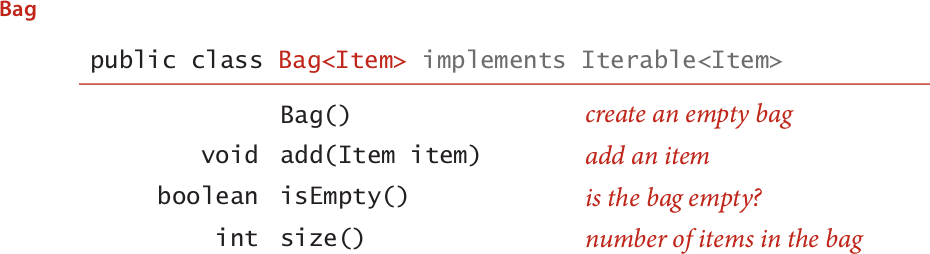
\includegraphics[width=0.8\textwidth]{Pics/API-Bag}

		\vspace{0.5cm}

		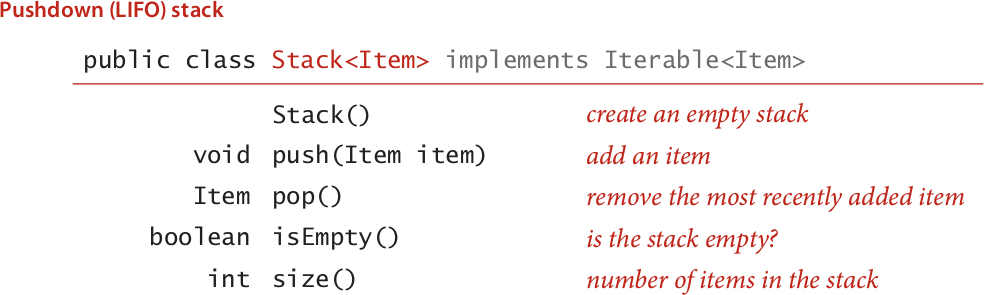
\includegraphics[width=0.8\textwidth]{Pics/API-Stack}

		\vspace{0.5cm}

		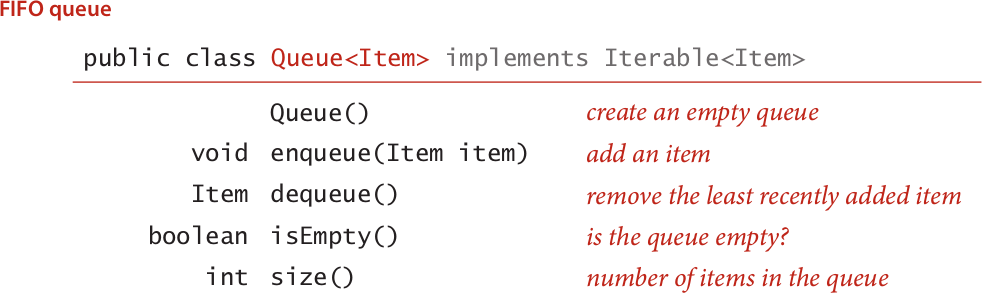
\includegraphics[width=0.8\textwidth]{Pics/API-Queue}

		\vspace{0.5cm}

		\hspace{2cm} 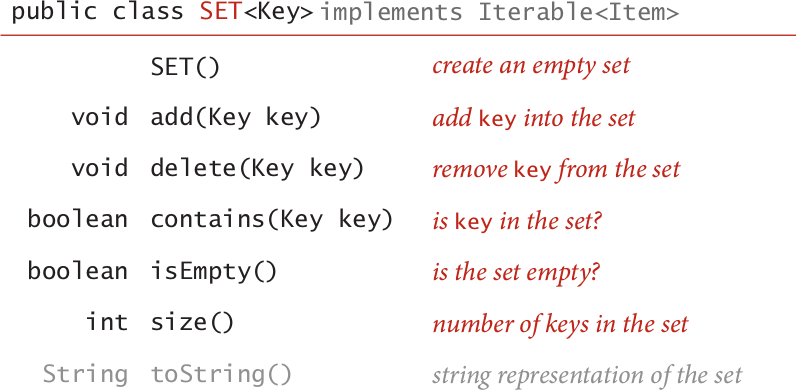
\includegraphics[width=0.7\textwidth]{Pics/API-SET}

		\vspace{1cm}

		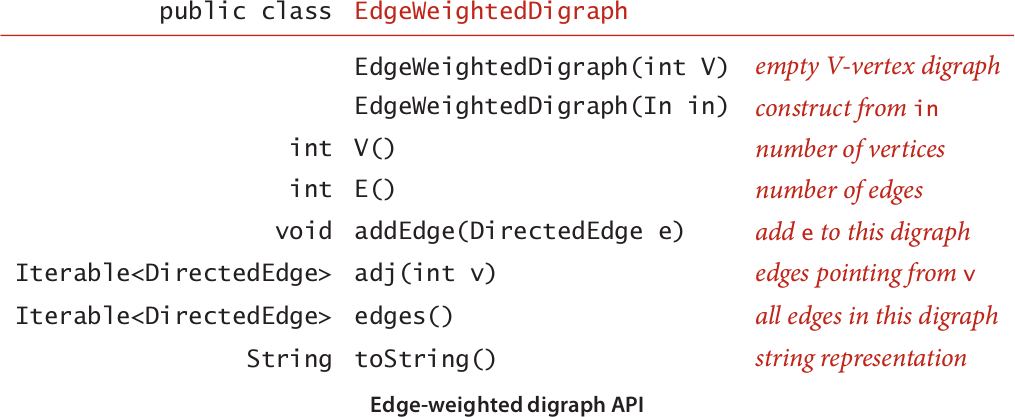
\includegraphics[width=0.8\textwidth]{Pics/API-EWDG}

		\vspace{1cm}

		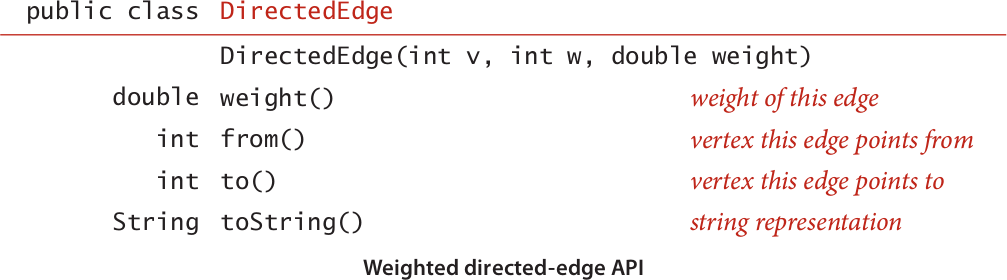
\includegraphics[width=0.8\textwidth]{Pics/API-DE}

		\vspace{1cm}

		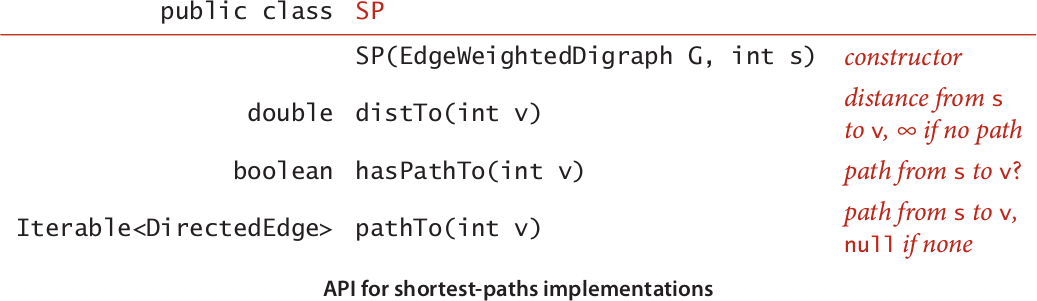
\includegraphics[width=0.8\textwidth]{Pics/API-SP}
	\end{center}


\end{questions}
\end{document}